\documentclass{tudphygp_eng}
\usepackage{tudphymd,mhchem}

% \documentclass[a4paper,11pt]{article}
\usepackage{color,supertabular,amsmath,amssymb}
\usepackage{cite}
\usepackage{array}
\usepackage{graphicx}
\usepackage{marvosym}
\oddsidemargin=0pt
\textwidth=460pt
\setlength{\textheight}{235mm}
\voffset=-1cm
% \headsep=0pt
\usepackage[english]{babel}

\versuch{Brownian motion}{BB}
\author{Dr. E. Lavrov, Thomas Fey}
\bearbeitet{engl. Dirk Bastin}{}
\date{Stand: 10.03.2015}







\begin{document}
\maketitle
%\begin{center}
%\includegraphics[scale=.17]{logo.eps}
%\end{center}          

%\vspace{5mm}
%\centerline{\bf\LARGE Brownian motion (BB)}

%\hline 
%\vspace{.5cm}
%\begin{center}
%\begin{tabular}{r@{:\quad}l}
%Standort & Institut f\"ur Angewandte Physik und Didaktik \\
%Supervising tutor & Dr. E. Lavrov \\  
%e-mail & {\tt edward.lavrov@physik.tu-dresden.de} \\
%Phone & 463 33637 \\
%Room & C115 \\
%Versuchsdauer &   8  Stunden \\ 
%Start & 8:00 o'clock 
%\end{tabular}
%\end{center}

\section{Introduction}

The Brownian motion was one of the first proofs of the thermal motion of molecules in liquids. In 1827, the botanist Brown investigated pollens in a water droplet. At first, he interpreted this motion as life force. Further investigations showed that the motion is also present in inanimate mater as consequence of collisions with the molecules of the liquid. The pollens collide with 10$^{21}$ collisions per second in the liquid. Every collision affects a force on the pollens and changes its momentum. Subsequently, the pollens are slowed down by friction with the molecules of the liquid. This process has no certain direction. In the average, the particles get the same displacements in each direction. The position of the particle does not change when it is investigated for a sufficient time. The Brownian motion belongs to this type of processes which need an adequate number of measurements to pass the detection limit. The measurement of e.g. the mass or acoustic waves can be perturbed by the Brownian motion.

\section{Schedule}

The goals of this practical course are the determination of 
\begin{itemize}
 \item the diffusion coefficient of the given combination of spherules and liquid, and
 \item the radius of the utilized spherules
\end{itemize}

Further, the constancy of the diffusion coefficient for different time intervals predicted by theory has to be proven.

\section{Theory}

In order to investigate the Brownian motion, the particles of the liquid are monitored by a microscope. The displacement of a particle during a certain time interval is measured. During the time interval $\tau$, the particle moves a statistically distributed different distance. Normally, the particle is restricted in one direction of motion during the measurement. $x_\tau$ and $y_\tau$ are utilized to represent the projections of the displacements of the particle along the two remaining dimensions. These projections are used to calculate the averages $x{_\tau}^2$ and $y{_\tau}^2$ of the squares of the projections of all distances passed within one time interval $\tau$. The motion of the particles seems randomly but the theory of statistical variations of A. Einstein and M. Smoluchowski shows that the diffusion coefficient
\begin{equation}
\label{eq:1}
D = \frac{\Delta x^2}{2\tau}
\end{equation}
is a constant for the given combination of spherules and liquid at a constant temperature. Since the positions of the axes are random there is no preferred direction within the x-y-plane. Thus, the mean of all $x{_\tau}^2$ and $y{_\tau}^2$ can be used for $x^2$. 

Since $D$ does not depend on the arbitrary choice of $tau$, ${x{_\tau}^2}/\tau$ has to remain constant under variation of $\tau$. This fact can be used to control the data series. To control the series, the values 
\begin{equation}
\label{eq:2}
 \Delta x_{2\tau}^2, \, \Delta x_{3\tau}^2, \, \ldots, \, \Delta x_{n\tau}^2
\end{equation}
has to be calculated using the obtained data. Having sufficiently exact and various data of the statistical motion of the particles (all having the same radius), the relation
\begin{equation}
\label{eq:3}
 \frac{\Delta x_\tau^2}{\tau}= \frac{\Delta x_{2\tau}^2}{2\tau} = \frac{\Delta x_{3\tau}^2}{3\tau} = \ldots = \frac{\Delta x_{n\tau}^2}{n\tau}
\end{equation}
has to be fulfilled. For this investigation, it is only necessary to prove the constancy up to $n=3$. Following A. Einstein and M. Smoluchowski, the diffusion coefficient can be calculated from
\begin{equation}
\label{eq:4}
 D=\frac{kT}{6\pi\eta r} . 
\end{equation}
\begin{tabular}{l@{\, -- \,}l}
$k$ & Boltzmann constant \\
$T$ & Temperature of the liquid \\
$\eta$ & Viscosity of the liquid \\
$r$ & radius of the particles within the liquid  
\end{tabular}

Prepare to derivate this formula. The radius of the particles of the Boltzmann constant can be determined by using (\ref{eq:1}) and (\ref{eq:4}) as long as one of the two values is known.

\section{Preparation of the specimen}

The specimen consists of a thin film of a suspension of microskopic spherules (Latex) which is positioned between an object plate and a cover glass. At first, the generation of the specimen is described. This and the appropriate cleaning works have to be done on the table. \emph{Tip}: A good preparation of a specimen is necessary for a successful experiment. The single-handed preparation of the specimen should provide first experiences for the evaluation of a suitable or an unsuitable specimens.

The preparation starts with the cleaning of the object plate and the cover glass using undenaturated ethanol and lint-free cloth. \emph{Important}: The cover glass is highly fragile! Always use index finger and thumb of one hand for cleaning.

The next step is the inspection of the suspension. It should be milky and free of clumpings and deposits. If the suspension contains deposits, then the suspension should be shaken. When the clumpings or/and deposits remain then a new suspension has to be produced. In this case, please ask the supervision tutor.

\begin{figure}[t]
\begin{center}
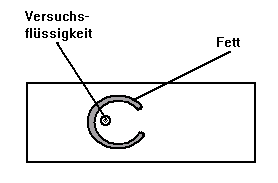
\includegraphics[width=.40\textwidth]{fig1.png} 
\caption{Object plate with an open circle of grease (\grqq{}Fett\grqq{}) and a droplet of the suspension (\grqq{}Versuchsfl{\"u}ssigkeit\grqq{})}
\label{fig1}
\end{center}
\end{figure}

\begin{figure}[t]
\begin{center}
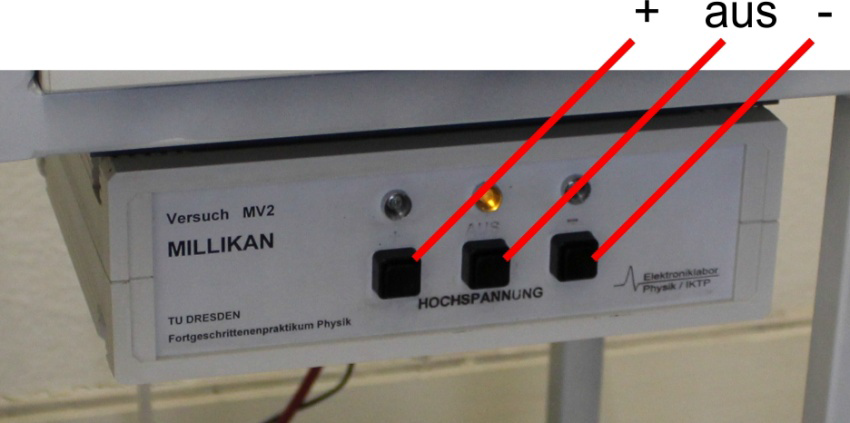
\includegraphics[width=.45\textwidth]{fig2.png} 
\caption{Covering of the circle of grease (\grqq{}Fett\grqq{}) by the cover glass (\grqq{}Deckglas\grqq{}) using a glass rod (\grqq{}Glasstab\grqq{}) and a pair of tweezers (\grqq{}Pinzette\grqq{})}
\label{fig2}
\end{center}
\end{figure}

During the following step, a non-closed circle of grease is pressed on the object plate. This is realized by using a plastic cylinder with an annular end which is covered with silicone grease taken from a grease box. A homogeneous distribution is achieved via turning of the plastic cylinder in the end cover of the grease box. The cylinder has an opening to ensure that the circle of grease is not closed completely.

During the following step, the plastic cylinder is pressed in the middle of the object plate whereas the opening of the plastic cylinder is aligned to the right side. The layer of grease should not be too thick since the particles should not be able to move within $z$-direction. Further, the generation of air pockets is possible which would superpose the Brownian motion by drift motions.

Now, a droplet of the suspension is laid on the object plate by using the glass rod. It is placed opposite to the opening of the circle of grease which schematically shown in Fig.~\ref{fig1}.

By using tweezers and the glass rod, the cover glass is oblique to the fat-free body apply even about the fat ring (see Fig.~\ref{fig2}). 

\begin{figure}[t]
\begin{center}
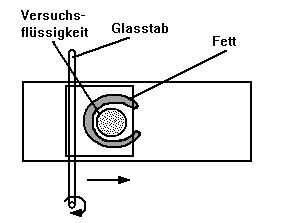
\includegraphics[width=.40\textwidth]{fig3.png} 
\caption{The cover glass is pressed onto the object plate via rolling of the glass rod.}
\label{fig3}
\end{center}
\end{figure}

Concluding, the cover glass is pressed onto the object plate. This is realized via rolling of the glass rod across the cover glass towards the opening of the grease ring for several times. This procedure should eliminate the air below the cover glass. The cover glass must not be moved. Possible leaked suspension liquid has to be dabbed or swept away with the glass rod. Finally, take some grease with a glass rod and close the opening of the grease ring from the outside.

\begin{figure}[h]
\begin{center}
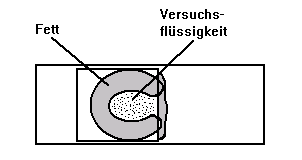
\includegraphics[width=.40\textwidth]{fig4.png} 
\caption{Schematic figure of a prepared specimen}
\label{fig4}
\end{center}
\end{figure}

\subsection{Experimental procedure}

\emph{Tip}: Before starting the microscope wait for the introduction given by the supervising tutor. Operating the microscope extreme caution! Do not use any force and do nor touch any optical faces!

Start the computer and create a new folder at \verb|D:\Versuch_BB\| which starts with YYYY-MM-DD (Year-Month-Day) followed by your group name. All the data - you will generate - will be saved in this folder which is named \grqq{}your folder\grqq{} in the upcoming text.

Before you can work with the microscope, you have to clean it using  propanol or ethanol. Then the darkfield condenser is installed. For this purpose, tune the nosepiece to the lowest magnification. Now inserting the condenser and clamp it. A droplet of immersion oil is placed centrally on the condenser. At next, the condenser is driven down a bit, so that it is located slightly below the sample plane. Now, if the specimen is placed, it must not touch the condenser. After fixation of the specimen through the terminals, the condenser is again gently lift until the immersion oil droplet touchs the object plate and spreads flat and without bubble formation. The condenser must not touch the specimen.

Now the lights has to be turned on and the specimen should be focused at the lowest magnification. The height of the condenser has to carefully adjusted that way, that an uniformly bright light spot in the specimen can be seen. When the light in the center is annular, the condenser is either too high or too low. Subsequently, the light spot is centered in the middle of the visual field. This is set with the centering ring and the lever of the condenser (see Fig.~\ref{fig5}). While tuning one element, you have to retain the other one. You should never perform the centering with the microscope mirror.

\begin{figure}[h]
\begin{center}
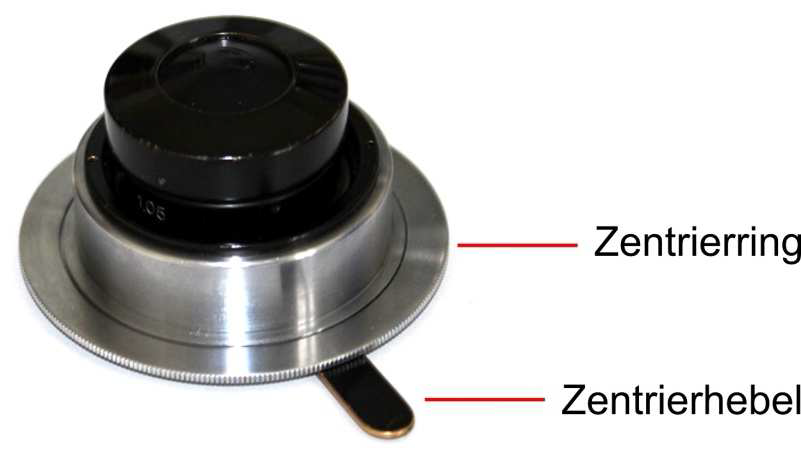
\includegraphics[width=.40\textwidth]{fig5.png} 
\caption{Dark field condenser with centering ring (\grqq{}Zentrierring\grqq{}) and lever (\grqq{}Zentrierhebel\grqq{})}
\label{fig5}
\end{center}
\end{figure}

\emph{Tip}: To facilitate the adjustment, the lens tube with the video camera can be temporarily replaced by the lens. Then go to higher magnifications and focus the specimen. The program TSO-VidMess on the computer was calibrated  for the lens having a 40x magnification. To prohibit a damage of the specimen and the lens during focusing, the lens is brought as close as possible to the specimen in lateral observation. It is important to make sure that the lens does not touch the specimen! Then you look at the specimen through the microscope and slowly increase the distance until the spherules in the liquid are in focus. Since the pursuit of the spherules in real time is a real challenge, it is more effective to record and save one or some videos in \grqq{}ffdshow\grqq{} format. A video should have a duration of 2-3~min and it should contain a lot of highly-visible spherules.

Then, the video can be played at a reduced speed. You select one of the moving highly-visible spherules in the center of the screen and mark its position in the program at equal time intervals. A zoom function can be used to increase the accuracy of the positions. The position should be tracked approx. every 3~s and between 10 and 20 data points should be recorded. After finishing a measurement series (right mouse button click), all recorded data become cached in a table (table symbol in the middle of the menu bar) by a double click with the left mouse button. This procedure can be repeated for an additional spherule from the video. The measured values are cached with a by one increased spherule number in the table by the program. If you have stored the paths of all spherules in this manner, then you save this file in tabular form (Selection of formatted text (\verb|*.txt|)) in your folder. Alternatively, you can save each spherule in a separate file. Overall, you should save the paths for at least 10 spherules. The following proposed analyze program works with one file per spherule. To do this, you choose a text editor, open one of the stored measurement files, and save all rows having a character string \grqq{}Punkt P\grqq{} and having the same spherule number in a separate file with a comprehensible file name (Proposal: \glqq{\verb|Spherule_No.txt|}\grqq) without changing the row structure in your folder that way to get at least 10 \grqq{}Single particle\grqq{} files. 

Finally, the temperature of the specimen has to be measured in which the room temperature is suitable. In order to correct the annealing done by the lights, 3~K have to be added to the measured room temperature. The values of viscosity can be taken from a provided table.

After finishing the experiment, all components polluted by immersion oil have to be cleaned using ethanol.

\section{Evaluation}

The way of evaluate your data is up to you. The program \grqq{}ORIGIN\grqq{} and a spreadsheet program are installed on the computer. The described and proposed evaluation will be done with the program HypraData (\verb|http://www.ssd.de/|). To start the program, the file \glqq{\verb|Auswertung_BB.ddd|}\grqq\ from the desktop has to be opened and saved in your folder. Every of your saved \grqq{}Single particle\grqq{} files is dragged into the empty database (Fig.~\ref{fig6}A) whereat every file should be dragged in a new table. You can switch between the table via using the green arrows in the menu bar. The evaluation database automatically calculates displacements, the squares of the shifts, the times between the measurement points, the diffusion coefficient, ... Figure \ref{fig6}B shows a filled table. The measured values are shown in column 2-4 ($\Delta t$, $x$, $y$). Here, a first overview concerning the measured values is given.

In the second step, rows must be corrected or extinguish from obvious false entries, respectively. These false entries can be seen distinctly in the picture \glqq{Darstellung der Bewegung}\grqq which can be opened via the tab \glqq{Brownsche Bewegung}\grqq. To do this, the entire row of the appropriate table has to be marked as shown in Fig.~\ref{fig6}B. Subsequently, the delete key (\grqq{}Entf\grqq{}) has to be pressed and \grqq{}Ja\grqq{} must be confirmed. The measured values can be scrolled by using  Page-up (\grqq{}Bild-Hoch\grqq{}) and Page-down (\grqq{}Bild-Runter\grqq{}) or the green arrows of the program. The rows containing false entries have to be deleted in every table. Finally, the temperature and viscosity with the associated error values have to be written in tab \glqq{Ergebnisse}\grqq\ (Fig.~\ref{fig6}A). In order to calculated the error value of the radius, you press \grqq{}Alt+u\grqq{} and set the number to 200 and confirm it by pressing \grqq{}Starten\grqq{} button.

All necessary diagrams are depicted in the other tabs. Is a diagram required for the protocol, you do a right click on the diagram \grqq{}Diagramm exportieren\grqq{}.

\emph{Tip}: Press \grqq{}Alt+L\grqq{} to open the menu to delete measured values. Double imported data have to be avoided.

%\newpage



%\newpage

\section{Questions about the experiment}

\begin{itemize}
\item What changes in a body, if it a quantity of heat is supplied?
 
\item Explain the Brownian motion. Think about why the Brownian motion limits the increase in the sensitivity of a scale or a galvanometer.

\item Which influences cause the transport phenomena diffusion, internal friction, and thermal conduction in gases? What magnitudes are transported there, and how does that happen?

\item What is suspension and sedimentation? What is the correlation between the molecule density and the potential energy of the particles in a sedimentation equilibrium? What is the \textit{H}-theorem of Ludwig Boltzmann?

\item Explain the 2. law of thermodynamics as law of probability!

\item Describe the structure of a microscope! Draw the ray path! What is the definition of the magnification of a microscope?

\item How does a dark field condenser work? 

\begin{figure}[h]
\begin{center}
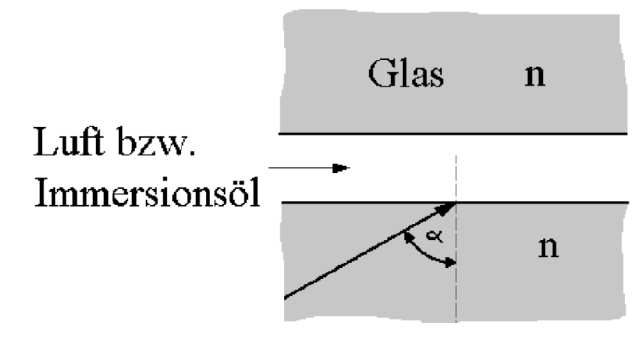
\includegraphics[width=.40\textwidth]{fig7.png} 
\caption{Slit between two glass (\grqq{}Glas\grqq{}) plates filled with air (\grqq{}Luft\grqq{}) oder immersion oil (\grqq{}Immersionsöl\grqq{})}
\label{fig7}
\end{center}
\end{figure}

\item How is the way of rays (Fig.~\ref{fig7}) in the case of $n$ sin $\alpha > 1$ ($n=1,5$), if the slit is filled with a) air or b) immersion oil ($n_I \approx 1,5$)?

\item At first, an object is viewed without and later with immersion oil between the speciment and the lens. Does the magnification change?

\item Why do we use dark field microscopy to investigate the Brownian motion?

\item Do we can see the spherules, if there is no immersion oil
\begin{enumerate}\itemsep=0pt
 \item between the condenser and the specimen or
 \item between the specimen and the lens?
\end{enumerate}

\item It is useful to replace $x^2$ by $|x|^2$ in (\ref{eq:1})?

\item In which case is it possible to combine data series from two different spherules?

\item Various spherules are investigated during the experiment. Which influence has a variation of the diameter of the spherule?

\item Which influences has a flux within liquid inside the grease ring for the determination of the Boltzmann constant? What could generate such a flow? Why do air bubbles within the specimen perturb the experiment?

\item Why is useful to absorb the thermal radiation before it enters the specimen? How can we determine experimentally whether the remaining thermal radiation still influences the experiment?

\item Are there other experiments which could prove the relation (\ref{eq:4}) ?

\end{itemize}

\section{Literature}

\begin{enumerate}
 \item G.~Loos, {\em Lehrbuch der Theoretischen Physik}, Leipzig: Akademische Verlagsgesellschaft Geest \& Portig KG, 1959. 
 
 \item B.~M.~Jaworski und A.~A.\ Detlaf, {\em Physik griffbereit}, Berlin: Akademie-Verlag, 1973. 
 
 \item A.~Einstein, \glqq{\em {\"U}ber die von der molekularkinetischen Theorie der W{\"a}rme geforderte Bewegung 
 von in ruhenden Fl{\"u}ssigkeiten suspendierten Teilchen}\grqq, Annalen der Physik 322, pp. 549--560, 1905. 
 
 \item K.~Prizibram, {\em Handbuch der Experimentalphysik}, Bd. VIII/2, Leipzig, 1929. 

\end{enumerate}

\section{Check list}

\renewcommand{\labelitemi}{\Large$\square$}
\begin{itemize}

 \item Clean the object plate and the cover glass
 \item Check the suspension if it contains clumping
 \item Generate a specimen
 \item Build in the dark field condenser
 \item Place the immersion oil correctly between condenser and specimen 
 \item Adjust the condenser (light beam centric and homogeneous)
 \item Focus the specimen with the microscope
 \item Record the video 
 \item Determine the temperature of the specimen
 \item Record 5--10 data series {\'a} 10--20 data points
 \item Evaluate of the data 
 \item Clean the measuring station and all used components

\end{itemize}

\begin{figure}[t]
\begin{center}
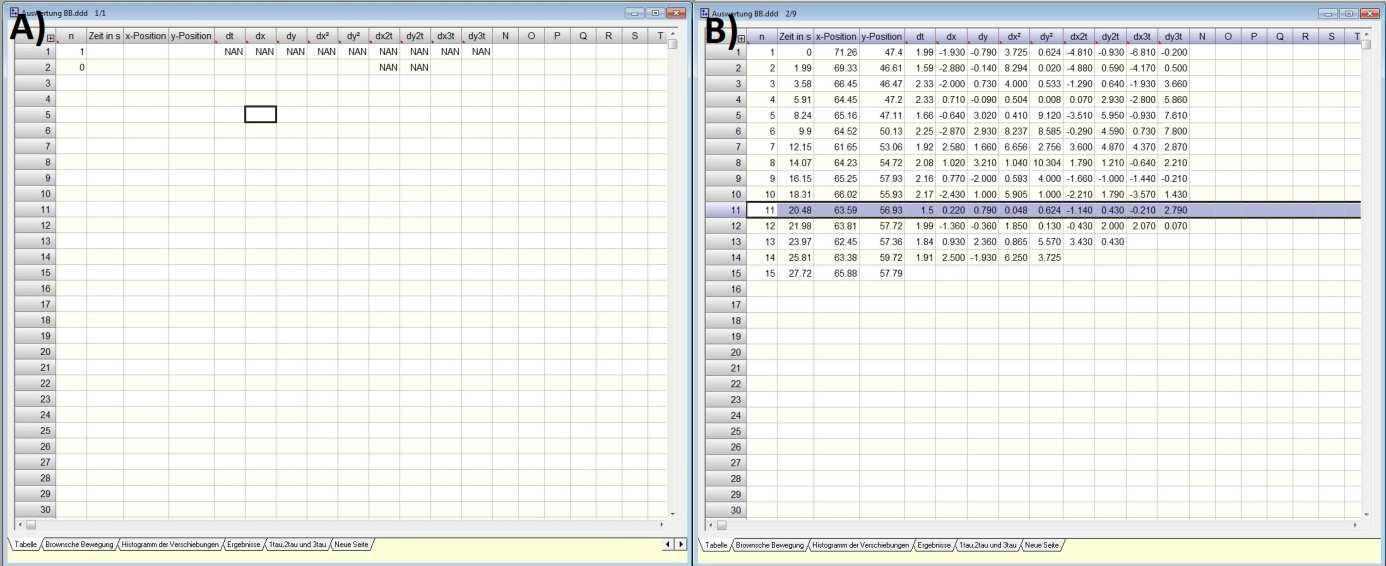
\includegraphics[width=1\textwidth]{fig6_1.png} 
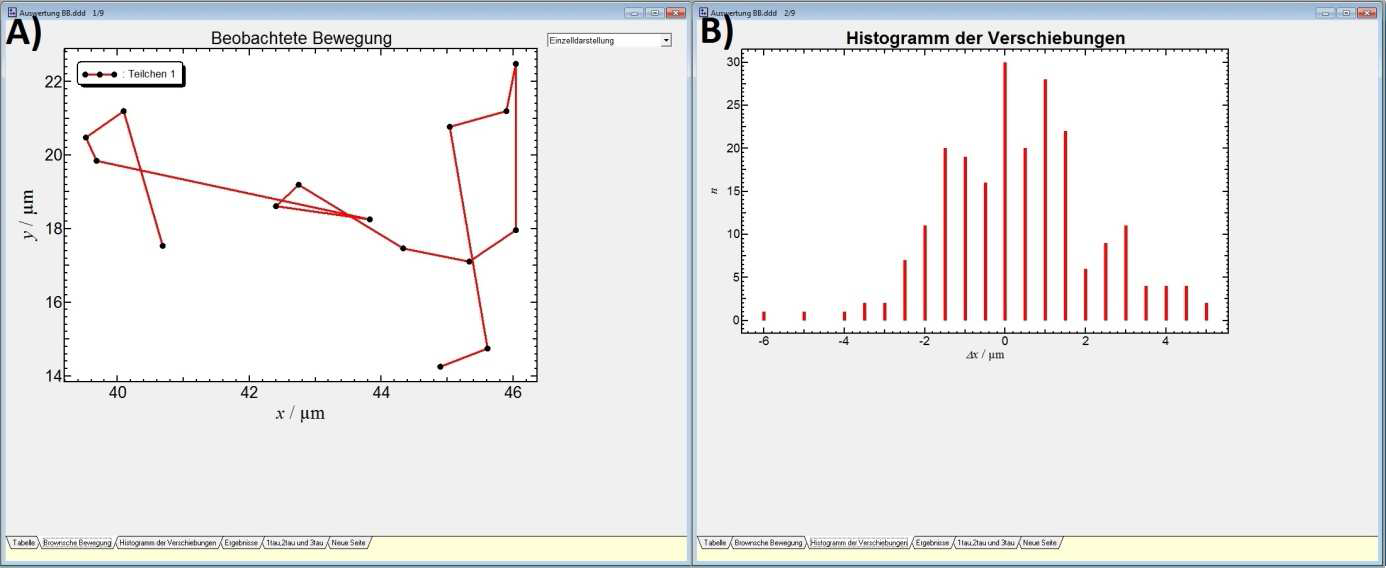
\includegraphics[width=1\textwidth]{fig6_2.png} 
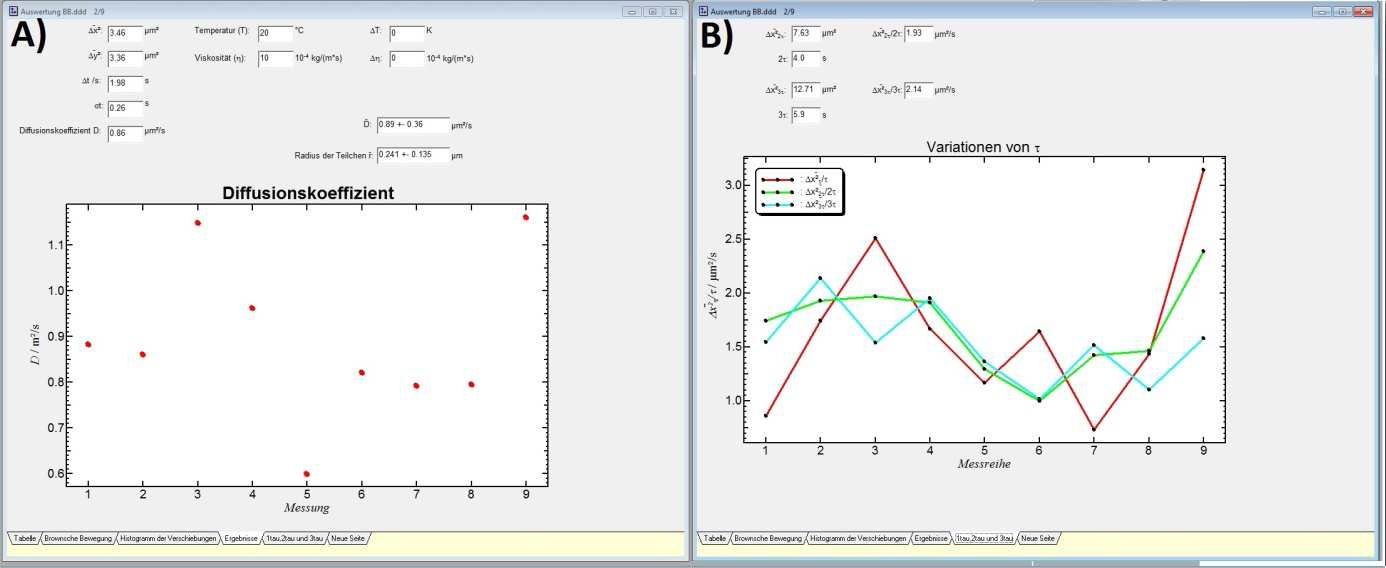
\includegraphics[width=1\textwidth]{fig6_3.png}
\caption{Top: A) empty and B) filled database \glqq{Auswertung BB.ddd}\grqq\ in tab \grqq{}Tabelle\grqq{}. Mid: \glqq{Auswertung BB.ddd}\grqq\ in tab A) Brownian motion \grqq{}Brownsche Bewegung\grqq{} and B) histogram of displacements \grqq{}Histogramm der Verschiebungen\grqq{}. Bottom: \glqq{Auswertung BB.ddd}\grqq\ in tab A) results \grqq{}Ergebnisse\grqq{} und B)  \glqq{1 tau, 2 tau und 3 tau}\grqq.}
\label{fig6}
\end{center}
\end{figure}

\end{document}